% !TEX TS-program = pdflatexmk
\documentclass[12pt]{article}
 \usepackage[margin=1in]{geometry} 
\usepackage{amsmath,amsthm,amssymb,amsfonts}
 \newtheorem{definition}{Definition}[section]
 \newtheorem{theorem}{Theorem}[section]
  \newtheorem{sats}{Sats}[section]
\usepackage[most]{tcolorbox}
\setlength{\parindent}{0.0in}
\setlength{\parskip}{0.05in}
\usepackage{empheq}
\usepackage{float}

\usepackage{framed}
\usepackage[most]{tcolorbox}
\usepackage{xcolor}
\colorlet{shadecolor}{orange!15}
\parindent 0in
\parskip 12pt
\geometry{margin=1in, headsep=0.25in}
\usepackage{amsthm}
\usepackage[utf8x]{inputenc}
\usepackage{comment}
\usepackage{xcolor}
\newcommand{\N}{\mathbb{N}}
\newcommand{\Z}{\mathbb{Z}}
\usepackage{graphicx}
\usepackage{pgf,tikz,pgfplots}
\pgfplotsset{compat=1.15}
\usepackage{mathrsfs}
\usetikzlibrary{arrows}
\usepackage{subcaption}
\pagestyle{empty}
\usepackage{systeme}
\usepackage{pgfplots}
\usepackage{hyperref}
\usepackage{amsthm} 
\newenvironment{solution}
  {\renewcommand\qedsymbol{$\blacksquare$}\begin{proof}[Solution]}
  {\end{proof}}
 
\usepackage[]{algorithm2e}

\newenvironment{problem}[2][Problem]{\begin{trivlist}
\item[\hskip \labelsep {\bfseries #1}\hskip \labelsep {\bfseries #2.}]}{\end{trivlist}}
%If you want to title your bold things something different just make another thing exactly like this but replace "problem" with the name of the thing you want, like theorem or lemma or whatever
\usepackage{mathtools}

%TO HIGHLIGHT USE \hl
\usepackage{xcolor}
\usepackage{soul}
\usepackage{bm}

\usepackage{epigraph}


\usepackage{dirtytalk}

\usepackage{mathtools}
\DeclarePairedDelimiter{\innerprod}\langle\rangle
\newcommand\conjinnerp[2][]{\:\overline{\mkern-4mu\innerprod[#1]{#2}\mkern-4mu}\:}
\usepackage{fancyhdr}
\pagestyle{fancy}
\fancyhf{}
\rhead{Machine Learning}
\lhead{Kiar Fatah}
\rfoot{Page \thepage}


\numberwithin{equation}{section}

\title{Machine Learning}

\author{Kiar Fatah}

\date{\today}
\begin{document}

\maketitle

\newpage

\tableofcontents 

\newpage
\epigraph{If you can’t explain something in simple terms, you don’t understand it.}{\textit{Richard Feynman }}
\newpage

\section{Lecture 2}
\subsection{Decision Tree}
A decision tree is a map of the possible outcomes of a series of related choices.
\subsection{How to build a Tree}
\begin{enumerate}
\item Choose the best question (according to the information
gain), and split the input data into subsets.
\item Terminate: call branches with a unique class labels leaves
(no need for further questions).
\item Grow: recursively extend other branches (with subsets bearing mixtures of labels).
\end{enumerate}

\subsection{How to ask the best questions?}
The machine will automate the questions for the decision tree, however how does it obtain the best questions to ask? It does so by with the help of Gini impurity and information gain.
\subsubsection{Gini impurity}
Gini impurity is a measurement of uncertainty in a node. It is calculated by how often a randomly chosen element from the set would be incorrectly labeled if it was randomly labeled according to the distribution of labels in the subset. 
\begin{equation}
    1 - \sum_i p_i^2.
\end{equation}
\subsubsection{Entropy}
Entropy is also a measurement of uncertainty in a node and can be applied instead of Gini impurity. It is calculated as
\begin{equation}
    \sum_i -p_ilog_2 p_i.
\end{equation}
The information entropy is measured in bits, corresponding to the logarithmic base 2. Tossing a coin results in the entropy 1, hence it has 1 bit of information. For a real dice and a fake dice the value is 2.58 and 2.16 bits of information respectively.

\subsubsection{Information gain}
Information gain is how much the question reduces the uncertainty. The information is given by the first set of values for the internal node subtracted by the average value of the impurity of the split set. 

\subsubsection{Best question}
The question with the \hl{highest value} on the information gain will be the one to ask.

\subsection{Overfitting}
Overfitting is when the learned models are overly specialised for the training samples. This occurs when the data is too noisy, not representative and when the model is too complex. This can be tackled by choosing a simpler model.

\subsubsection{Pruning}
The idea of reduced error pruning is to consider each node in the tree as a candidate for removal. A node is removed if the resulting pruned tree performs at least as well as the original tree over a separate validation dataset. The pruning is done on validation set, until it is harmful for the model.

\subsubsection{Validation set}
Due to pruning there is a need for validation dataset that is not training nor test data set. Therefore if there is access to a rich data set, it is separated to three categories. In essence the validation set is used to estimate prediction error for model selection (i.e. to determine hyperparameters).

\section{Lecture 3}

\subsection{Introduction}
How does one determine the right model, f, from the data? The simple concept for classification is by calculating the misclassification rate in consideration to the data. Assume the following data is given $\mathcal{D} = {(\vec{x_1},y),....}$ is given. The misclassification rate is given by
\begin{equation}
err(f,\mathcal{D}) = \frac{1}{N}\sum Ind(f(\vec{x}) \neq y)
\end{equation}

\subsection{Curse of Dimensionality}
\begin{enumerate}
    \item Easy problems in low-dimensions are harder in high-dimensions, e.g training more complex models with limited sample data.
    \item In high-dimensions everything is far from everything else, this is an issue in the nearest neighbour model, this causes issues with Nearest Neighbours.
    \item Any method that attempts to produce locally varying functions in small isotropic neighbourhoods will run into problems in high dimensions.
\end{enumerate}


\subsection{The Bias-Variance Trade-off}
Let us imagine we could repeat the modelling for many times – each time by gathering new set of training samples, D. The resulting models will have a range of predictions due to randomness in the underlying data set.
\begin{enumerate}
    \item Variance: Refers to the amount by which $\hat{f}$, the prediction function, would change if we estimated it using a different training data set.
    \item Bias: Refers to the error that is introduced by approximating a real-life problem, which may be extremely complicated, by a much simpler model.
\end{enumerate}
This can be showcased in figure \ref{var_bias}
\begin{figure}[!ht]
    \centering
    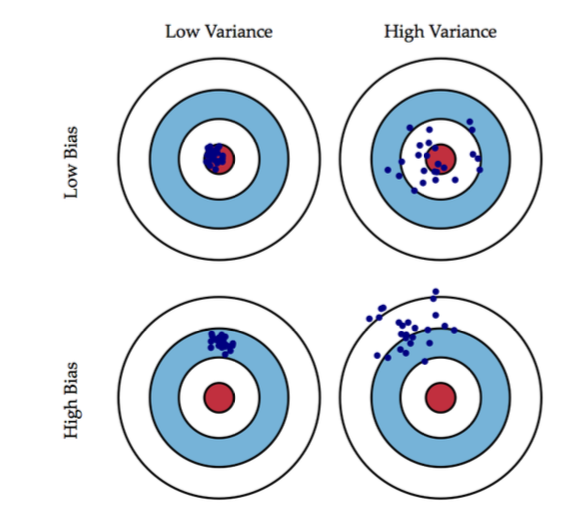
\includegraphics[scale = 0.7]{var_bias.png}
    \caption{Variance versus Bias}
    \label{var_bias}
\end{figure}
In essence the relationship between complexity, bias and variance can be summarised as
\begin{enumerate}
    \item Low model complexity implies high bias, low variance.
    \item High model complexity implies low bias, high variance.
\end{enumerate}
Note that bias and variance are equally important as we are always dealing with a single realisation of the data set.

\section{Lecture 4}

\subsection{Linear Regression, A Parametric Method}
Simple linear regression assumes theres a linear relationship between the output and input. Therefore a linear equation is assumed, parametric method. However, the coefficients are unknown and thus needs to be approximated. 

The measurement of error is mean square. It is a convex function. Therefore the coefficients that minimises the sum of the squared error is given by the vector that sets the gradient of the sum of squared error to zero.

\begin{equation}
E_{in} (w) = ||Xw - Y ||^2 \implies \frac{\partial E_{in}}{\partial w} =  2X^T(Xw - Y) = 0 \implies w = (X^T X )^{-1}X^T Y
\end{equation}
whereas w is the coefficients, X the data, Y the label and $E_{in}$ the sum of squared errors.
\subsection{RANdom SAmpling Consensus}
Random sampling consensus or RANSAC is applied when the data set S contains outliers
\begin{enumerate}
    \item Randomly select a (minimum number of) sample of s data
    points from S and instantiate the model from this subset.
    \item Determine the set of data points $S_i$ which are within a distance threshold t of the model. The set $S_i$ is the consensus set of samples and defines the inliers of S.
    \item If the subset of $S_i$ is greater than some threshold T, re-estimate the model using all the points in Si and terminate
    \item If the size of $S_i$ is less than T, select a new subset and repeat the above.
    \item After N trials the largest consensus set $S_i$ is selected, and the model is re-estimated using all the points in the subset $S_i$
\end{enumerate}
In essence RANSAC
\subsection{Disadvantages with RANSAC}
\subsection{Differences with Parametric and Non-parametric Methods}
\begin{enumerate}
    \item If the parametric form is close to the true form of f, the parametric approach will outperform the non-parametric
    \item As a general rule, parametric methods will tend to outperform non-parametric when there is a small number of observations per predictor (i.e. in a high dimension).
    \item Interpretability stand point: Linear regression preferred to KNN if the test MSEs are similar or slightly lower.
\end{enumerate}
\subsection{k-NN Regression, A Non-parametric}
The k-NN regression method is closely related to the k-NN classifier. Given a value for K and a prediction point $x_0$, k-NN regression first identiffies the K training observations that are closest to $x_0$ represented by $N_0$. It then estimates $f(x_0)$ usin the average of all the training responses in $N_0$. In other words
\begin{equation}
    \hat{f(x_0)} = \frac{1}{K} \sum_{x_i \in N_0} y_i.
\end{equation}
Note larger values of k provide a smoother and less variable fit (lower variance!)
\subsection{Parametric or Non-parametric Methods?}
\begin{enumerate}
    \item  If the parametric form is close to the true form of f, the parametric approach will outperform the non-parametric
    \item As a general rule, parametric methods will tend to outperform non-parametric when there is a small number of observations per predictor (i.e. in a high dimension).
    \item Interpretability stand point: Linear regression preferred to KNN if the test MSEs are similar or slightly lower.
\end{enumerate}
\subsection{Shrinkage Methods}
A common way to fit models is by appling least square, however an alternative is it is possible to fit a model containing all p predictors using a technique that constrains or regularizes the coefficient estimates, or equivalently that shrinks the coefficient estimates towards zero.
\begin{enumerate}
    \item Among a large number of variables X in the model there are generally many that have little (or no) effect on Y
    \item Leaving these variables in the model makes it harder to see the big picture, i.e. the effect of the “important variables”
    \item Would be easier to interpret the model by removing unimportant variables (setting the coefficients to zero)
\end{enumerate}
\subsection{Ride Regression}
Similar to least squares but minimizes different quantity
\begin{enumerate}
    \item Shrinkage penalty
    \item The parameter $\lambda$
    \item Interpation of the graphs
    
\end{enumerate}
\subsection{The Lasso}
Similar to ridge regression but with slightly different term














































\end{document}